\documentclass[border=3pt,tikz]{standalone}
% Shared look for every TikZ figure in these notes.
% Included by each standalone figure file; also keeps the figures consistent
% with the colours used in the PDF and on the website.

\usepackage{tikz}
\usepackage{pgfplots}
\pgfplotsset{compat=1.18}
\usetikzlibrary{arrows.meta, decorations.markings, decorations.pathmorphing,
                patterns, calc, positioning}
\usepackage{amsmath}

% Series colours are the three validated categorical slots also used by the
% interactive widgets, so a path drawn in the printed notes and the same path on
% the website are the same colour. They clear the colour-vision-deficiency and
% contrast checks as a set; every path is direct-labelled as well, so colour is
% never the only thing carrying identity.
\definecolor{duPurple}{HTML}{68246D}
\definecolor{duBlue}{HTML}{2A78D6}
\definecolor{duRed}{HTML}{EB6834}
\definecolor{duGreen}{HTML}{1BAF7A}
\definecolor{duGrey}{HTML}{6B6B6B}

\tikzset{
  axisline/.style   = {-{Stealth[length=3mm]}, line width=0.7pt, black},
  path1/.style      = {duBlue,   line width=1.1pt},
  path2/.style      = {duRed,    line width=1.1pt},
  path3/.style      = {duGreen,  line width=1.1pt},
  statedot/.style   = {circle, fill=black, inner sep=1.4pt},
  arrowhead/.style  = {decoration={markings,
                        mark=at position #1 with {\arrow{Stealth[length=2.6mm]}}},
                       postaction={decorate}},
  lbl/.style        = {font=\small},
  slbl/.style       = {font=\footnotesize, duGrey},
  workfill/.style   = {duPurple, opacity=0.16},
}

\begin{document}
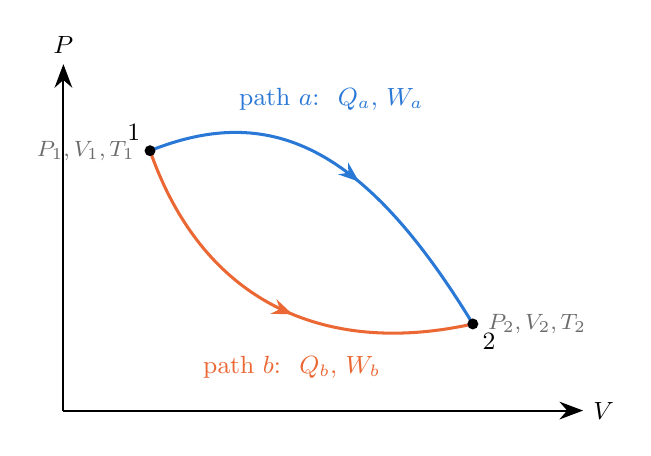
\begin{tikzpicture}[scale=1]
  \draw[axisline] (0,0) -- (6.6,0) node[right, lbl] {$V$};
  \draw[axisline] (0,0) -- (0,4.4) node[above, lbl] {$P$};

  \coordinate (s1) at (1.1,3.3);
  \coordinate (s2) at (5.2,1.1);

  \draw[path1, arrowhead=0.55] (s1) .. controls (2.6,3.9) and (3.8,3.4) .. (s2);
  \draw[path2, arrowhead=0.55] (s1) .. controls (1.8,1.3) and (3.4,0.7) .. (s2);

  \node[statedot] at (s1) {};
  \node[statedot] at (s2) {};

  \node[lbl, above left=0pt and 0pt] at (s1) {1};
  \node[lbl, below right=0pt and 0pt] at (s2) {2};
  \node[slbl, left=2pt] at (s1) {$P_1,V_1,T_1$};
  \node[slbl, right=2pt] at (s2) {$P_2,V_2,T_2$};

  \node[lbl, duBlue] at (3.4,3.95) {path $a$:\; $Q_a,\,W_a$};
  \node[lbl, duRed]  at (2.9,0.55) {path $b$:\; $Q_b,\,W_b$};
\end{tikzpicture}
\end{document}
